%%% Local Variables:
%%% mode: latex
%%% TeX-master: "../main"
%%% End:

\part{Methodology}\label{methodology}
This section outlines the implementation details of the voxel rendering engine, starting with the selection of programming languages and libraries, reviewing the engine's architecture, and diving deep into the data structures and algorithms employed. It particularly focuses on VDB for voxel representation and the optimization of ray-casting algorithms.
Finally, this section will discuss the extension of these algorithms to full-fledged ray tracing, allowing for dynamic lightning and glossy material support.

\section{Language and framework}
\hyphenation{WebGPU}

The voxel rendering engine is built using \textbf{Rust}, a programming language known for its focus on safety, speed, and concurrency\supercite{rustbook}.
Rust's design emphasizes memory safety without sacrificing performance, making it an excellent choice for high-performance applications like a rendering engine.
The language's powerful type system and ownership model prevent a wide range of bugs, making it ideal for managing the complex data structures and concurrency challenges inherent in rendering engines. Thanks to this, no memory leak or null pointer was ever encountered throughout the development of this project.

For the graphical backend, the engine utilizes \textbf{wgpu}\supercite{wgpu:doc}, a Rust library that serves as a safe and portable graphics API. wgpu is designed to run on various backends, including Vulkan, Metal, DirectX 12, and WebGL, ensuring cross-platform compatibility. This API provides a modern, low-level interface for GPU programming, allowing for fine-grained control over graphics and compute operations. wgpu is aligned with the WebGPU specification\supercite{webgpu:doc}, aiming for broad support across both native and web platforms, using the WebGPU shading language (wgsl)\supercite{wgsl:doc}. This choice ensures that the engine can leverage the latest advancements in graphics technology while maintaining portability and performance.

The combination of Rust and wgpu offers several advantages for the development of a rendering engine:

\begin{enumerate}
  \item \emph{Safety and Performance:} Rust's focus on safety, coupled with wgpu's design, minimizes the risk of memory leaks and undefined behaviours, common issues in high-performance graphics programming. This added safety is thanks to Rust's idea of zero-cost abstractions.

  \item \emph{Cross-Platform Compatibility:} With wgpu, the engine is not tied to a specific platform or graphics API, enhancing its usability across different operating systems and devices.

  \item \emph{Future-Proofing:} wgpu's adherence to the WebGPU specification ensures that the engine is built on a forward-looking graphics API designed to be efficient, powerful, and broadly supported. It also allows the future option of supporting web platforms once browsers adopt WebGPU more thoroughly.

  \item \emph{Concurrency:} Rust's advanced concurrency features enable the engine to efficiently utilize multi-core processors, crucial for the heavy computational demands of rendering pipelines.
\end{enumerate}

These technical choices form the foundation for building the voxel rendering engine. Following this, the engine's architecture is designed to take full advantage of Rust's performance and safety features and wgpu's flexible, low-level graphics capabilities, setting the stage for implementing advanced voxel representation techniques and optimized ray tracing algorithms.

\section{Engine architecture}

\begin{figure}[H]
  \centering
  \includesvg[width=0.8\linewidth]{architecture}
  \caption[Engine architecture]{Data flow from \texttt{.vdb} object file to rendering an image on the screen, dotted lines represent functionality handled by the \texttt{winit} crate.}
\end{figure}

The engine's operation centres around an event-driven main loop that blocks the main thread.
This loop processes various events, ranging from keyboard inputs to redraw requests, and updates the window, context, and scene accordingly, routing each event to its corresponding handler.

\begin{figure}[H]
  \centering
  \includesvg[width=0.8\linewidth]{engine_1}
  \caption[Egine event loop]{Engine event-loop diagram. Dotted arrows are implemented by the \texttt{winit} crate. Black lines represent the flow of events. The orange arrow represents the the GPU context's render function called on the scene, for the window.}
\end{figure}


\subsection{Runtime}
\newacronym{os}{OS}{Operating System}
\begin{samepage}
At the engine's core sits \texttt{Runtime}  structure, which manages the interaction between its main components:
\begin{itemize}
  \item The \texttt{Window} is a handler to the engine's graphical window. It is used in filtering \acrshort{os} events that are relevant to the engine, grabbing the cursor and other boilerplate.
  \item The \texttt{Wgpu Context} handles the creation and application of the rendering pipeline.
  \item The \texttt{Scene} contains information about the camera, environment and a container voxel data structure.
\end{itemize}
\end{samepage}

\begin{lstlisting}[language=rust,caption={Runtime definition},captionpos=b]
pub struct Runtime {
  context: WgpuContext,
  window: Window,
  scene: Scene,
}

impl Runtime {
  ...
  pub fn main_loop(&mut self, event: Event, ...) {
    match event {
      ...
    }
  };
}
\end{lstlisting}


For example, window events (e.g. keyboard \& mouse input) generally modify the scene, like the camera position, and therefore are routed to the \verb|Scene| struct.

Another key event is the \verb|RedrawRequested| event, which signals that a new frame should be rendered. It is routed to the wgpu context to start the rendering pipeline.

The \verb|RedrawRequested| event is emitted in \verb|Runtime|, and when it receives the \verb|MainEventsCleared| event, it schedules the window for a redraw.

\subsection{Window}
The \verb|Window| data structure, included in the \textbf{winit}\supercite{winit:doc} crate, handles window creation and management and provides an interface to the GUI window through an event loop. This event loop is what \verb|Runtime|'s main loop is mounted on.

The interaction between the \verb|Window| and the \verb|Runtime| forms an event-driven workflow. The window emits events, and the runtime manages and distributes these events accordingly, forming a feedback loop.

\subsection{Scene}\label{scene:def}
The \verb|Scene| data structure holds information about the environment being rendered; this includes the model, camera, and engine state.

\begin{lstlisting}[language=rust,caption={Scene definition},captionpos=b]
pub struct Scene {
    pub state: State,
    pub camera: Camera,
    pub model: VDB,
}
\end{lstlisting}

This section covers the camera and state implementation, and the model will be covered later \cref{vdb:sec} when discussing the \acrshort{vdb} implementation.
\newacronym{fps}{FPS}{Frames per second}
\newacronym{fov}{FOV}{Field of view, explained in \cref{scene:def}, \cref{fov:def}}

\paragraph{State} handles information about the engine state, such as cursor state and time synchronising to decouple engine events from the \acrshort{fps} (e.g. camera movement should not be slower at lower FPS).

\paragraph{Camera} describes all the elements needed to control and represent a camera:
\begin{enumerate}
    \item \emph{Eye:} The camera's position in the 3D space acts as the point from which the scene is observed.
    \item \emph{Target:} The point in space the camera is looking at determines the direction in which the camera is pointed.
    \item \emph{Field of View (FOV):} An angle representing the range that is in view. It refers to the implementation's FOV on the $Y$ (vertical) axis.\label{fov:def}
    \item \emph{Aspect ratio:} The ratio between the width and height of the viewport. It ensures that the rendered scene maintains the correct proportions.
\end{enumerate}
The eye and target are updated when moving the camera through a \verb|CameraController| struct that handles keyboard and mouse input. The FOV and aspect ratio are set based on the window proportions to avoid distortion. The way in which this camera information is used will be detailed in \cref{gputypes}, which covers what information is actually sent to the GPU in compute shaders.


\subsection{WgpuContext}
The \verb|WgpuContext| structure is the backbone of the rendering pipeline in the voxel rendering engine. It contains the necessary components for interfacing with the GPU using the wgpu API, managing resources such as textures, shaders, and buffers, and executing rendering commands.

Broadly, \verb|WgpuContext| has the following responsibilities:
\begin{enumerate}
  \item \emph{Initialisation:} The constructor sets up the wgpu instance, device, queue, and surface.
        It also configures the surface with the desired format and dimensions, preparing the context for rendering.
  \item \emph{Resource Setup:} The constructor prepares various resources such as textures for the atlas representation of VDB data, uniform buffers for rendering state, and bind groups for shader inputs.
        It also dynamically reads VDB files, processes the data, and updates GPU resources accordingly.
  \item \emph{Rendering:} The render method updates the window surface.
        It triggers compute shaders for voxel data processing, manages texture and buffer updates, and executes the render pipeline. Additionally, it manages shader hot-reloading, renders the developer GUI and handles screen capture for recording.
\end{enumerate}

\subsection{Graphics Pipeline}
This section provides an overview of the graphics pipeline initiated at a \verb|RedrawRequest| event.

\begin{figure}[H]
\noindent\begin{minipage}[t]{0.75\textwidth}
  \vspace{0.5cm}
  When the \verb|WgpuContext|'s render method is invoked, it starts by obtaining a reference to the output texture and creates a corresponding view. Following this, a command encoder is initialised to record GPU commands.

  Next, it uses the \verb|FrameDescriptor|, a structure designed to transform scene information (including the model, camera, and engine state) stored on the CPU into GPU-compatible bindings. This step prepares all necessary bindings for the compute shaders, executing the ray-tracing algorithm across distributed workgroups, with the results written to a texture.

  Once the computation is complete, the rendered image's texture is prepared for display. This process involves creating a vertex shader to generate a full-screen rectangle, onto which the texture is rasterised using fragment shaders, effectively transferring the rendered image to the output texture.

  The final phase involves adding the GUI layer over the rendered scene before presenting the completed output texture on the screen.
\end{minipage}
\hfill
\begin{minipage}[t]{0.24\textwidth}
  \vspace{-0.5cm}
  \begin{figure}[H]
    \centering
    \includesvg[width=\linewidth]{pipeline}
  \end{figure}
\end{minipage}
\end{figure}

\subsection{GPU Types}\label{gputypes}
This section covers the \verb|FrameDescriptor| data structure and how it generates GPU bindings from the data in \verb|Scene|, which is stored on the CPU.

Virtually the entire ray-tracing algorithm is run in compute shaders, meaning all the information about the model, camera, lights, and metadata must be passed through to the GPU.

The statically sized data, i.e. the camera, sunlight and metadata, is passed in a uniform buffer. This buffer is assembled inside the \verb|FrameDescriptor|, which wraps \verb|ComputeState|.

\begin{lstlisting}[language=rust]
#[repr(C)]
pub struct ComputeState {
  view_projection: [[f32; 4]; 4],
  camera_to_world: [[f32; 4]; 4],
  eye: [f32; 4],
  u: [f32; 4],
  mv: [f32; 4],
  wp: [f32; 4],
  render_mode: [u32; 4],
  show_345: [u32; 4],
  sun_dir: [f32; 4],
  sun_color: [f32; 4],
}
\end{lstlisting}

The GPU's uniform binding system has strict requirements regarding the types and sizes of data that can be passed to shaders. Therefore, information must be packed into memory-aligned bytes. This is facilitated by the \#[repr(C)] attribute, which organizes the struct's layout to match that of a C struct. The data also needs to be padded to fit the aligment options, for that reason all fields are 16 bytes, even if they carry less information.

\begin{lstlisting}[language=rust,caption={\texttt{ComputeState} build method that transforms CPU data into GPU-ready data},captionpos=b,
  label={cstate:build}]
impl ComputeState {
  ...
  pub fn build(
    c: &Camera,
    resolution_width: f32,
    render_mode: RenderMode,
    show_grid: [bool; 3],
    sun_dir3: [f32; 3],
    sun_color3: [f32; 3],
    sun_intensity: f32,
    ) -> Self;
}
\end{lstlisting}

The role of \verb|ComputeState| is to translate high-level CPU structures onto these low-level GPU types. In future sections, the function of the structure fields will be thoroughly detailed.

\subsection{Camera}

This section explains how the 3D ray-casting camera is implemented. In a ray-tracing engine, a camera casts rays from its eye through the middle of the pixels and into the scene.

Fundamentally, the role of the camera is to convert points from world space into screen space. To that end, a view projection matrix can be constructed from the camera's properties (eye, target, \acrshort{fov}, aspect ratio) that take any point in world space and project it onto camera space.

In order to cast a ray in world space from the camera's eye through the middle of the pixel and into the scene, we need to bring the pixel from screen space into world space. This is the inverse operation of projection, and hence, the projection matrix's inverse matrix is the camera-to-world matrix.

\begin{align}
  \bm{d_{s}} = \begin{bmatrix}
              x - \frac{\rm{width}}{2} \\
              \frac{\rm{height}}{2} - y \\
              -\frac{h}{2}\tan^{-1}{\frac{\rm{fov}}{2}} \\
            \end{bmatrix},
  \ \rm{C2W} = \begin{bmatrix}
                  u_{x} & v_{x} & w_{x} \\
                  u_{y} & v_{y} & w_{y} \\
                  u_{z} & v_{z} & w_{z} \\
                \end{bmatrix}
\end{align}
\begin{align}
\intertext{Multiplying gives the pixel coordinates in world space}
  \bm{d_{w}} =
      \begin{bmatrix}
        x - \frac{\rm{width}}{2} \\
        \frac{\rm{height}}{2} - y \\
        -\frac{h}{2}\tan^{-1}{\frac{\rm{fov}}{2}} \\
      \end{bmatrix}
      \begin{bmatrix}
         u_{x} & v_{x} & w_{x} \\
         u_{y} & v_{y} & w_{y} \\
         u_{z} & v_{z} & w_{z} \\
      \end{bmatrix}
         &=
      \begin{bmatrix}
        (x - \frac{\rm{width}}{2})u_{x} + (\frac{\rm{height}}{2} - y)v_{x} - w_{x}\frac{h}{2}\tan^{-1}{\frac{\rm{fov}}{2}} \\
        (x - \frac{\rm{width}}{2})u_{y} + (\frac{\rm{height}}{2} - y)v_{y} - w_{y}\frac{h}{2}\tan^{-1}{\frac{\rm{fov}}{2}} \\
        (x - \frac{\rm{width}}{2})u_{z} + (\frac{\rm{height}}{2} - y)v_{z} - w_{z}\frac{h}{2}\tan^{-1}{\frac{\rm{fov}}{2}}
      \end{bmatrix}
\intertext{Which can be re-written by factoring out constant terms into $\bm{w'}$:}
  \bm{d_{s}} &= x\bm{u} + y*(-\bm{v}) + \bm{w'} \\
  \bm{w'} &= -\bm{u}\frac{\rm{width}}{2} + \bm{v}\frac{\rm{height}}{2} - \bm{w}\frac{h}{2}\tan^{-1}{\frac{\rm{fov}}{2}}
\end{align}

This form of the ray direction equation is very useful since the vectors $\bm{u}, \bm{v}$ and $\bm{w'}$ can all be computed once per frame, and then the equation is applied in compute shaders per pixel. This method is explained in more detail in this article\supercite{camera_rays}.

\crefformat{lstlisting}{lst. #2#1#3}
\Crefformat{lstlisting}{Lst. #2#1#3}

In the implementation, the calculation of these constant vectors is the responsibility of the \verb|ComputeState| data structure; the \verb|build| method (\cref{cstate:build}) takes in a \verb|Camera| specified by its eye, target, \acrshort{fov} and aspect ratio, and computes the view projection matrix, inverts it to get the camera to world matrix, extracts $\bm{u}, \bm{v}$ and $\bm{w}$, then uses the screen's resolution to calculate $\bm{w'}$. It then packs these vectors into 16-byte arrays.

\subsection{Shaders}
This section explains the role of the three shader stages in the implementation.

\begin{multicols}{2}
  \paragraph{Compute Shaders} are the first in the pipeline. They are responsible for performing the entire ray-tracing algorithm. The Compute shader distributes computational power to work groups, which can be considered independent units of execution that handle different parts of the calculation in parallel.
  Each work group is made up of multiple threads that can execute concurrently, significantly speeding up the process by allowing multiple computations to occur simultaneously.
  The Compute Shader casts rays from the camera eye through the pixels; intersections with the model determine a pixel's colour based on material properties and record these results on a 2D texture.

  \begin{figure}[H]
    \centering
    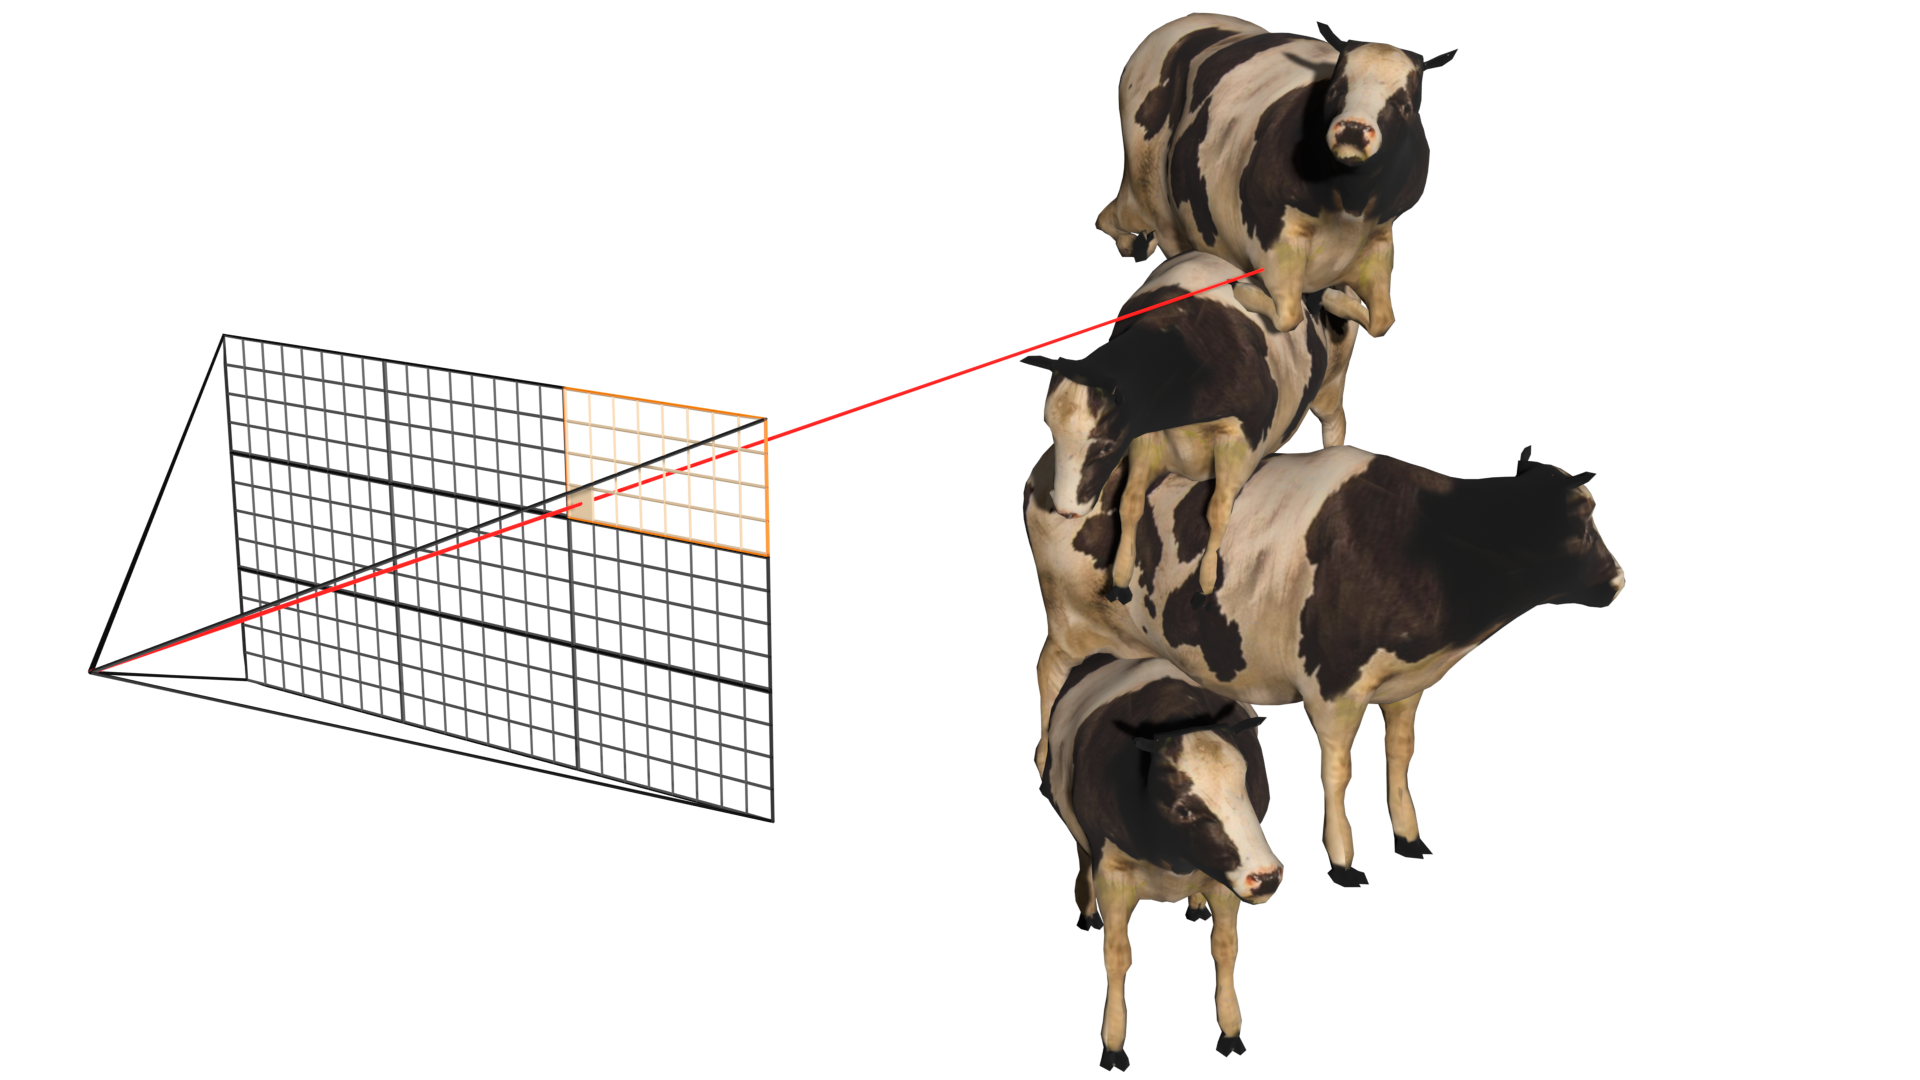
\includegraphics[width=1.2\linewidth]{compute_shaders}
    \caption[Compute shader visualization]{Compute shader worker casting a camera ray through a pixel. Workgroups of size $8\times4\times1$ have split up the screen.}
  \end{figure}
\end{multicols}
\paragraph{Vertex Shaders} follow Compute Shaders in the graphics pipeline. Their main role is to define the vertices of a screen-sized rectangle, which serves as the canvas for overlaying the texture computed in the Compute Shader stage.
\paragraph{Fragment Shaders} are the last shaders in the pipeline. The Fragment Shaders' role is to rasterize the texture onto the full-screen rectangle prepared by the Vertex Shader. This step effectively transfers the texture onto the display window.
\begin{multicols}{2}
  \begin{figure}[H]
    \centering
    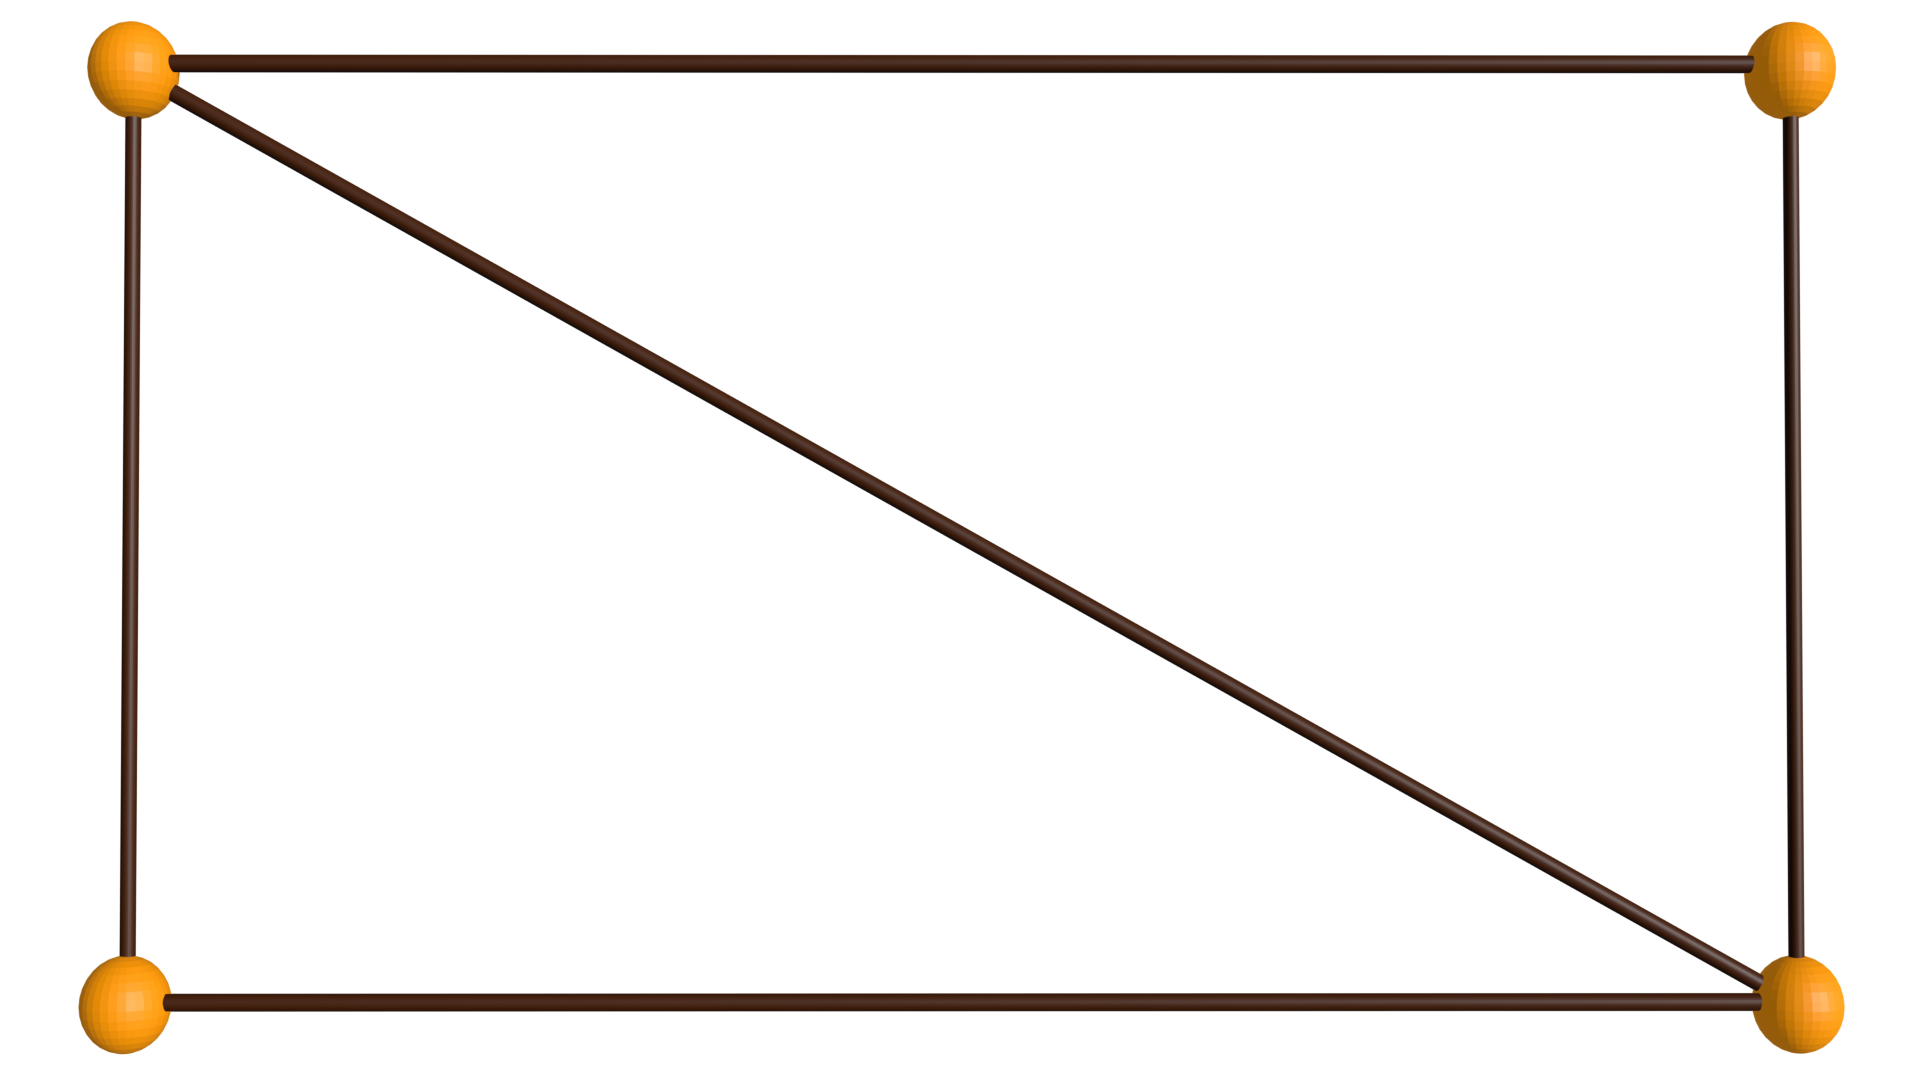
\includegraphics[width=0.8\linewidth]{vertex_shaders}
    \caption[Vertex shader visualization]{Vertex shader creating the output surface}
  \end{figure}

  \begin{figure}[H]
    \centering
    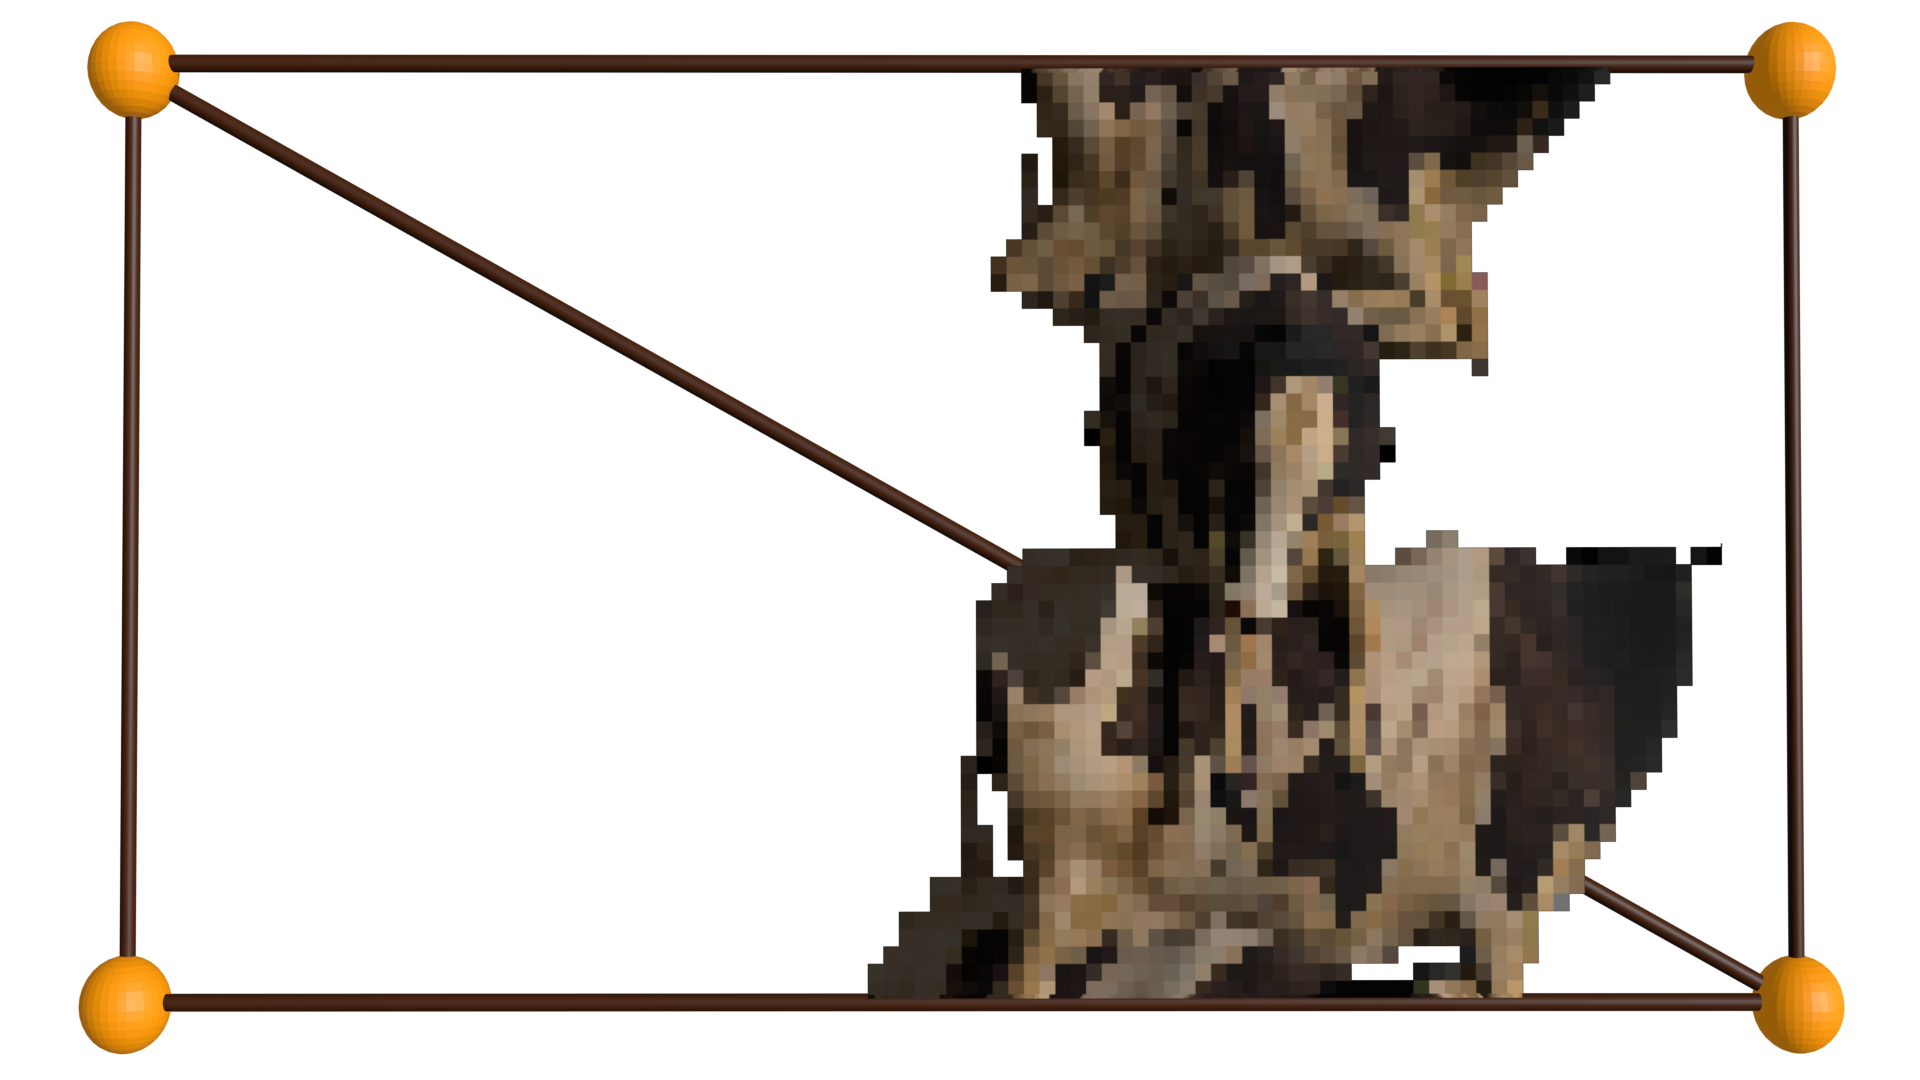
\includegraphics[width=0.81\linewidth]{fragment_shaders}
    \caption[Fragment shader visualization]{Fragment shader rasterizing the compute shader texture onto the output surface}
  \end{figure}
\end{multicols}

\subsection{GUI}
\newacronym{gui}{GUI}{Graphical User Interface}

This section covers the implementation of the \acrshort{gui} that allows the scene to active model to be changed and lighting to be modified, but also provides helpful developer metrics like ms/frame and other benchmarks.

The GUI is managed using the \verb|egui| crate\supercite{egui:doc}.
\verb|egui| is an immediate\supercite{im_gui} mode GUI library, which contrasts with traditional retained-mode GUI frameworks\supercite{im_vs_rt}.

In immediate mode, GUI elements are redrawn every frame and only exist while the code that declares them is running. This approach makes \verb|egui| flexible and responsive, allowing quick updates and changes without needing to manage a complex state or object hierarchy.

The GUI code is run as part of the graphics pipeline in the following steps:
\begin{enumerate}
\item \emph{Start Frame:} Each frame begins with a start-up phase where \verb|egui| prepares to receive the definition of the GUI elements. This setup includes handling events from the previous frame, resetting the state as necessary, and preparing to collect new user inputs.

\item \emph{Define GUI Elements:} The application defines its GUI elements by calling functions on an \verb|egui| context object. These functions dynamically create widgets such as buttons, sliders, and text fields based on the current state and user interactions. This step is where the immediate mode shines, as changes to the GUI's state are made directly in response to user actions without requiring a separate update phase.

\item \emph{End Frame:} After all GUI elements are defined, the frame ends with \verb|egui|, rendering all the GUI components onto the screen. During this phase, \verb|egui| computes all elements' final positions and appearances based on interactions and the layout rules provided.

\item \emph{Integration with Graphics Pipeline:} The GUI is overlaid on the application using a texture that \verb|egui| outputs. As in the previous section, this texture is drawn over the application window using a simple full-screen quad.
\end{enumerate}

\subsection{Recording}

The engine includes an integrated screen recorder designed to efficiently capture screen footage without compromising the frame rate. Unlike external tools such as OBS, which must capture screen output externally and can be slow due to their inability to access application internals, this engine captures the output texture directly before it is displayed on the screen. This method significantly reduces the time required for capture, giving smoother results and keeping the frame rate high.

\begin{figure}[H]
  \centering
  \includesvg[width=0.6\linewidth]{recording}
  \caption[Recording thread diagram]{Producer-Consumer pattern of screen recording implementation}
\end{figure}

This process's key aspect is ensuring that texture transfer and video encoding are handled asynchronously on a separate thread. This is done using a Producer-Consumer pattern, where the main thread acts as the producer. It periodically places frames into a blocking queue. From this queue, an encoding thread, acting as the consumer, retrieves and processes the frames, encoding them into PNG format and feeding them into \verb|ffmpeg|, a video encoding utility. This approach ensures background processing, minimizing the impact on the engine's performance.

\subsection{VDB Implementation}

In this section the theory and implementation the VDB data structure is covered.

The VDB (Volumetric Dynamic B-tree) is an advanced data structure designed for efficient and flexible representation of sparse volumetric data. It is organized hierarchically, consisting of root nodes, internal nodes, and leaf nodes, each serving distinct purposes within the structure. This section begins by explaining in detail how VDB is structured, and it continues by going though the implementation of the data structure in the rendering engine.

\subsubsection{Data Structure}
VDBs are sparse, shallow trees with a fixed depth but expandable breadth, capable of covering an virutally infinite spatial domain. This design enables the VDB to efficiently manage large and complex datasets by adjusting the level of detail dynamically and minimizing memory usage.

\begin{figure}[H]
  \centering
  \includegraphics[width=\linewidth]{vdb}
  \caption{2D \& 1D slices of the VDB data structure representing three quarters of a circle. Top left: 2D dense representation of the circle. Top right: 2D sparse representation of the VDB. Bottom left: Sparse representation of the 1D vdb. Usually, VDB nodes have many more child nodes, which whould make it harder to visualise, hence a smaller version of VDB is shown. This figure is an augumented version of the one in the original paper\supercite{vdb2013}}
\end{figure}

At the hear of the data structure are its three types of nodes, internal root and leaf. The VDB data structure is inherently general, each of the nodes' sizes can be modefied depending on the application. However, in practice only one specialization of the VDB structure is used, that is the VDB345. This is because the authors of the original paper\supercite{vdb2013} analyized a suite of possible shapes and sizes, and this configuration of VDB the most balanced between performance and memory footprint for most practical applications [TODO: what applications?]

\paragraph{Leaf Nodes} They are the lowest level in the tree structure. They store a 3D cubed grid of side length $2^{\log_{2} D}$ (i.e. only powers of 2). An leaf value in the grid can be a voxel's data, other associated data for empty values (such as SDF information), or an empty value.
Leaf nodes also store a value mask. This is a bit-array meant to compactly determine if value at a specific coordinate in the 3D grid is voxel data or an empty value.

In the implementation the trait \verb|Node| is defined which gives some associated data and methods leaf and internal nodes have.

\begin{lstlisting}[language=rust,caption={\texttt{Node} trait definition},captionpos=b,label={code:node}]
pub trait Node {
    /// LOG2_D of side length
    /// LOG2_D = 3 => `512 = 8 * 8 * 8` values
    const LOG2_D: u64;
    /// Total conceptual LOG2_D node
    const TOTAL_LOG2_D: u64;
    /// Total conceptual LOG2_D of child node
    const CHILD_TOTAL_LOG2_D: u64 = Self::TOTAL_LOG2_D - Self::LOG2_D;
    /// Side length
    const DIM: u64 = 1 << Self::LOG2_D;
    /// Total conceptual dimension
    const TOTAL_DIM: u64 = 1 << Self::TOTAL_LOG2_D;
    /// Size of this node (i.e. length of data array)
    const SIZE: usize = 1 << (Self::LOG2_D * 3);
    /// Total conceptual size of node, including child size
    const TOTAL_SIZE: u64 = 1 << (Self::TOTAL_LOG2_D * 3);
}
\end{lstlisting}

In \cref{code:node}, \verb|TOTAL_LOG2_D| represents the $\log_{2}$ of the total dimension of the node, meaning how much actual space the node occupies. Leaf nodes are at the bottom of the tree and don't have children so this is the same as $\log_{2} D$, but this value will be relevant for internal nodes. All other attributes are determined at compile-time depending on the size of the node $\log_{2} D$.

\begin{quote}
  \paragraph{Sidenote on Coordinate Systems}

  It is very convenient for side lengths to be powers of two because of the way integers are stored in memory, as binary values. To get the global coordinate of a node with \verb|TOTAL_LOG2_D| $= 3$ that contains a point in global coordinates, the 3 least signifcant bits of each coordinate have to be masked out. This can essentially be done in a single CPU instruction for each coordinate.

\begin{lstlisting}[language=rust]
/// Give global origin of Node coordinates from `global` point
fn global_to_node(global: GlobalCoordinates) -> GlobalCoordinates {
    global.map(|c| (c >> Self::TOTAL_LOG2_D) << Self::TOTAL_LOG2_D)
}
\end{lstlisting}

Simillary, to get the relative coordinates of a global point within the node are precisely the \texttt{TOTAL\_LOG2\_D} least siginificant bits.

\begin{lstlisting}[language=rust]
/// Give local coordinates relative to the Node containing `global` position
fn global_to_relative(global: GlobalCoordinates) -> LocalCoordinates {
    global.map(|c| (c & ((1 << Self::TOTAL_LOG2_D) - 1)))
}
\end{lstlisting}

This pattern of a few bit-wise operations can acheive any conversion from between coordinate systems one might need, and all of these through operations are extremly fast to compute on modern CPUs.
\end{quote}

\Cref{code:leaf} shows a simplified definition of the leaf node data structure in the implementation. It has two fields: data which is an array representing the 3D cube grid of values, and value mask which is a the bit-mask carrying information on what each value represnts, a voxel or empty space. the data array has has $2^{3\log_{2} D}$ entries(e.g. for $\log_{2} D = 3 \Rightarrow D = 8$ the leaf node has $8\times8\times8 = 512 = 2^{9}$ values). The value mask has the same number of bit entries, but it is stored as an array of unsined 64 bit integers, hence there are $\frac{D^{3}}{64}$ of them.

\begin{lstlisting}[language=rust, captionpos=b, caption={
    \texttt{LeafNode} definition.
    In the original paper\supercite{vdb2013} node data is set as a union instead of a enum, in order to save on memory space, only using the masks to determine the type of a particular values.
    In this implementation a enum is used strictly for \emph{ergonomics}, as the extra 1 byte of memory per value is generally not expensive on heap allocated memory.
    The value mask will still be curcial for the GPU version of VDB where there is more need for effective memory management and shading languages do not have enum support.
    In the \texttt{Node} trait implementation, since these nodes are the bottom level in the hierarchy (meaning they have no children), their in-memory dimensions are the same as their world space dimensions.
  }, label{code:leaf}]
pub struct LeafNode<ValueType, const LOG2_D: u64>
{
    pub data: [LeafData<ValueType>; (1 << (LOG2_D * 3))],
    pub value_mask: [u64; ((1 << (LOG2_D * 3)) / 64)],
}

pub enum LeafData<ValueType> {
    Tile(usize),
    Value(ValueType),
}

impl<ValueType, const LOG2_D: u64> Node for LeafNode<ValueType, LOG2_D>
{
    const LOG2_D: u64 = LOG2_D;
    const TOTAL_LOG2_D: u64 = LOG2_D;
}
\end{lstlisting}

The implenetation is general both in the type of value that is stored at the voxel level, \verb|ValueType|, and in the dimension of the Node, \verb|LOG2_D|. This makes use of Rust's generic const expresions feature \supercite{rust:generic} that is only available on the nightly toolchain. These work in a way akin to C++ templates allowing to define types of static size chosen by the user of the data structure that are resolved at compile time. This approach effectively allows to costumize the tree breadth and depth at compile time with no run-time overhead.

\paragraph{Internal Nodes} They sit between the root node and the leaf nodes, forming the middle layer of the tree structure.
They also store a 3D cubed grid of side length $2^{D}$ of values. An internal value can either be a pointer to a child node (leaf or internal), or a tile value, which is a value that is the same for the whole space that would be covered by a child node in that position.
Internal nodes also store a value mask and child mask. These determine if value at a specific coordinate in the 3D grid is child pointer, value type or empty value.


\begin{lstlisting}[language=rust, captionpos=b, caption={
    \texttt{InternalNode} definition. Internal nodes have an extra field, the child mask that is the same size of the value mask.
    Aditionally the internal data enum now has variants for a child pointer or 4 bytes of memory.
}]
pub struct InternalNode<ValueType, ChildType: Node, const LOG2_D: u64>
{
    pub data: [InternalData<ChildType>; (1 << (LOG2_D * 3))],
    pub value_mask: [u64; ((1 << (LOG2_D * 3)) / 64)],
    pub child_mask: [u64; ((1 << (LOG2_D * 3)) / 64)],
}

pub enum InternalData<ChildType> {
    Node(Box<ChildType>),
    Tile(u32),
}

impl<ValueType, ChildType: Node, const LOG2_D: u64> Node
    for InternalNode<ValueType, ChildType, LOG2_D>
{
    const LOG2_D: u64 = LOG2_D;
    const TOTAL_LOG2_D: u64 = LOG2_D + ChildType::TOTAL_LOG2_D;
}
\end{lstlisting}

When implemening the \verb|Node| the \verb|TOTAL_LOG2_D| is calculated by adding this nodes $\log_{2}D$ with the child node's total $\log_{2}D$.
For example, for an internal node with $log_{2}D = 4$ with children that are leaf nodes of $log_{2}D' = 3$, the internal node's $\log_{2}D_{{total}}$ will be $7$. This means that the internal node has $16\times16\times16$  children that each have $8\times8\times8$ voxels; the total number of voxels one of these internal nodes is $128\times128\times128$ or $2^{7}\times2^{7}\times2^{7}$.

It is imporant to note that all children of an internal node must be of the same type, which means each level in the tree only has one type of node, this ensure consistency in the coordinate system discussed previously.

\paragraph{Root Node} The root node is a single node at the top of the VDB hierarchy. Unlike typical nodes in a tree data structure, the root node in a VDB does not store data directly but instead serves as an entry point to the tree.
It contains a hash map indexed by global coordinates, linking to all its child nodes. This setup allows for quick access and updates, as the root node acts as a guide to more detailed data stored deeper in the hierarchy. Because its children nodes are stored by a hash map, it only stores information about space that has information to be stored(unlinke an octree where empty top level nodes are frequent). The root node's primary role is to organize and provide access to internal nodes.


\begin{lstlisting}[language=rust, captionpos=b, caption={
    \texttt{RootNode} definition. \texttt{RootData} is either a pointer to a child or a 4 bytes of data for a tile value.
  },label={code:root}]
pub struct RootNode<ValueType, ChildType: Node>
{
    pub map: HashMap<GlobalCoordinates, RootData<ChildType>>,
}

pub enum RootData<ChildType> {
    Node(Box<ChildType>),
    Tile(u32),
}
\end{lstlisting}

Finally, a VDB simply consits of a root node and some metadata associated with the volume, stored in the \verb|grid_descriptor| feild. This metadata is generally only imprtant when reading enad writing \verb|.vdb| files.

\begin{lstlisting}[language=rust, captionpos=b, caption={\texttt{VDB} definition}]
pub struct VDB<ValueType, ChildType: Node>
{
    pub root: RootNode<ValueType, ChildType>,
    pub grid_descriptor: GridDescriptor,
}
\end{lstlisting}

\subsubsection{VDB345}
$\rm{VDB}345$ is the most widely used configuration of the VDB data structure, because gives a good balance of performance and memory footprint for most applications.
\begin{sloppypar}
  To refer to different shapes of the VDB data structure, by convention, they are named as ${\rm{VDB}[a_{0},a_{1},\dots, a_{n}]}$, meaning it has a  bottom layer of leaf nodes with $\log_{2}D_{0}=a_{0}$ follwed by $n$ layers of internal nodes with $\log_{2}D_{i}=a_{i}$. $\rm{VDB}345$ therfore with leaf nodes with $\log_{2}D_{n3} = 3$ and two layers of internal nodes, one with $\log_{2}D_{n4} = 4$ and the other with $\log_{2}D_{n5} = 5$.
\end{sloppypar}

To implement this type of VDB new type name for each type of node is created as show in \cref{vdb345}, chaining them up the tree. This section will refer to these nodes as \texttt{Node3}s, \texttt{Node4}s and \texttt{Node5}s respectively.

\begin{lstlisting}[language=rust, captionpos=b, caption={\texttt{VDB345} definition}, label={vdb345}]
pub type N3<ValueType> = LeafNode<ValueType, 3>;
pub type N4<ValueType> = InternalNode<ValueType, N3<ValueType>, 4>;
pub type N5<ValueType> = InternalNode<ValueType, N4<ValueType>, 5>;
pub type VDB345<ValueType> = VDB<ValueType, N5<ValueType>>;
\end{lstlisting}

To calculate how much the in-memory size, in bytes, of each node the follwing calculation can be done, by taking into account the size of the 3D grid together with the masks:
\begin{align*}
&\text{For leaf nodes:}& M &= D^{3} (v + 1) + \frac{D^{3}}{8} \\
&\text{For internal nodes (2 masks):}& M &= D^{3} (v + 1) + 2\frac{D^{3}}{8} \\
&\text{Where:}& D &= \text{dimension of node (side-length)} \\
&& v &= \text{number bytes the value type occupies (min. of 4)}
\intertext{Simillarly to find out how many voxels each node covers in world space:}
  &\textbf{Node3:}& D &= 2^3 = 8 \\
  && S &= D^3 = 8\times8\times8 = 512 \\
  &\textbf{Node4:}& D &= 2^4 = 16 \\
  && D_{t} &= 2^{4+3} = 128 \\
  && S &= D_{t}^3 = 128\times128\times128 = 2,097,152 \\
  &\textbf{Node5:}& D &= 2^5 = 32 \\
  && D_{t} &= 2^{5+4+3} = 4096 \\
  && S &= D_{t}^3 = 4096\times4096\times4096 = 68,719,476,736
\end{align*}

A single Node5 represent $4069^3$ voxels in space, just under $69$ billion.
This is where the power of the VDB data structure can be seen; models can have multiple \verb|Node5|s covering trillions of voxels in total all of which can be acessed in $O(1)$ time, by going three layers down the tree.


\subsubsection{Reading \texttt{.vdb}}
VDB was introduced along with an associated file format \verb|.vdb| which gives a compact representation of the data structure. In this section the part of the implementatio that reads VDB files and stores them into memory is covered.

\subsubsection{Computing SDF}
\subsubsection{GPU VDB}

%%% Local Variables:
%%% mode: latex
%%% TeX-master: "../main"
%%% End:

\section{Ray tracing}
With the structure of the rendering engine and the primary data structure covered, it is time to bring everything together to construct an image.
A ray tracing algorithm is required, first needing an algorithm to cast a ray.
This section will cover methods for casting rays and ray-tracing algorithms, as well as how these integrate with the VDB data structure to optimise performance.

\subsection{Casting a ray}
The background section glossed over a suite of ray-casting algorithms.
This section will detail the implementation of three such algorithms, all built on top of each other: DDA, HDDA, and HDDA+SDF.

\subsubsection{DDA}
\acrshort{dda} works by ray marching from grid intersection to grid intersection, ensuring each voxel is only polled once.
The starting values are a source point and a normalised direction vector.
\begin{enumerate}
  \item Initial Position (ipos): The starting position of the ray within the voxel grid, calculated by flooring the source vector. It gives the indices of the voxel grid where the ray starts.
  \item Delta Distance (deltaDist): This calculates how far the ray must travel in each axis to cross a voxel boundary. It is computed by dividing the length of the direction vector (dir) by each component of the direction vector, giving the distance the ray travels in each axis per step.
  \item Step (step): A vector determining the direction to step through the grid in each axis (i.e., whether to increment or decrement the index in each dimension). It is determined by the sign of the direction vector components.
  \item Side Distance (sideDist): This vector stores the distance the ray needs to travel to hit the next side of a voxel. It starts with the distance to the first boundary from the source position, adjusted by half a voxel size in the direction of travel to ensure the calculation centres within a voxel.
\end{enumerate}

The core idea of the algorithm is that it precomputes the amount one unit of movement on either axis causes the ray to progress (\texttt{deltaDist}). It then maintains a record of how far the ray has progressed on each axis and selects the one for which the ray has moved the least, i.e. the closest boundary intersection.

\begin{lstlisting}[language=rust, captionpos=b, caption={\texttt{DDA} algorithm}]
const MAX_RAY_STEPS: i32 = 64;
fn cast_ray_dda(src: vec3<f32>, dir: vec3<f32>) -> vec3<f32> {
  var ipos = vec3<i32>(floor(src));
  let deltaDist = abs(vec3<f32>(length(dir)) / dir);
  let step = vec3<i32>(sign(dir));
  var sideDist = (sign(dir) * (vec3<f32>(ipos) - src) + (sign(dir) * 0.5) + 0.5)
    * deltaDist;
  var mask = vec3<bool>(false);

  for (var i: i32 = 0; i < MAX_RAY_STEPS; i++) {
    let val = getVoxel(ipos);
    if (val.hit) {
      return val.color + dot(vec3<f32>(mask) * vec3(0.01, 0.02, 0.03), vec3(1.0));
    }

    var b1 = sideDist.xyz <= sideDist.yzx;
    var b2 = sideDist.xyz <= sideDist.zxy;
    mask = b1 & b2;

    sideDist += vec3<f32>(mask) * deltaDist;
    ipos += vec3<i32>(mask) * step;
  }

  return vec3<f32>(dir);
}
\end{lstlisting}

Specifically, at each iteration of the ray marching loop, three operations are performed:
\begin{enumerate}
  \item Voxel Check: At each step, the algorithm checks whether the current voxel (ipos) is occupied by using the getVoxel(ipos) function. If this function returns true, indicating a hit, the loop exits as the ray has intersected a voxel, and its colour, adjusted to distinguish between the face on which the ray hit, is returned.
  \item Boundary Calculation: Determines which voxel boundary (x, y, or z) will be hit next by comparing the distances in sideDist. The logic here involves comparing each component of sideDist against the others to find the smallest value. This is computed using vector comparisons b1 and b2, which are boolean vectors.
  \item Update sideDist and ipos: Updates the current side distance and position based on which boundary will be hit next. For example, If the smallest distance is in the x-direction, then the x-component of sideDist and ipos are updated.
\end{enumerate}

\subsubsection{HDDA}
This section covers the Hierarchical DDA specifically tailored for traversing volumetric data represented in a VDB, using the data structure at last. This method is much more effective in handling large and sparse volumetric datasets due to its hierarchical traversal mechanism, which significantly enhances computational efficiency and scalability.

The key idea is to scale the ray step at each iteration by the lowest level of detail at that point. For example, at a point in an empty Node4, there is no reason not to step directly the side length of a Node4 along an axis since it is guaranteed that there is no voxel data in that node.

The following is a breakdown of the algorithm in \cref{hdda:code}:
\paragraph{Initialisation}
\begin{enumerate}
  \item The ray's initial position \texttt{p} is set to the source point src.
  \item The \texttt{step} vector determines the traversal direction in the grid is the non-zero sign of the ray.
  \item The \texttt{step01} vector is used as a flag to determine whether the size on a given axis should be added when calculating step candidates.
        It essentially discriminates between the cases shown in \cref{hdda:fig}.
  \item The \texttt{idir} vector represents the inverse of the directional vector.
        \newacronym{fpu}{FPU}{Floating-Point Unit, a coprocessor for handling floating point numbers}
        It is precomputed to avoid doing element-wise division in the loop's body since multiplication is faster than division on \acrshort{fpu}s.
  \item The \texttt{mask} has the same role as in standard DDA; it will be used to decide which increment produced the smallest step on the ray.
\end{enumerate}
With this initial information, the ray can start marching along the VDB.

\begin{figure}[H]
  \centering
  \includesvg[width=0.6\linewidth]{hdda}
  \caption[HDDA iteration diagram]{
    \texttt{HDDA} iteration. (a): Ray positive on both axes.
    When a ray direction has a positive component, because of the directionality of the modulo operation, it must be subtracted from the size of the node to maintain the ray direction.
    (b): Ray negative on both axes. When a ray has a negative component, the modulo must simply be inverted since the size is already accounted for. \\
    Blue and grey vectors are candidate steps at the given iteration; each has its components outside the squares.
    The blue vector has to be selected since it is the shorter one.
    The black vector represents the modulo-size vector. The $\odot$ operation denotes element-wise multiplication.
    A small branching factor is not typical of the VDB data structure; this was chosen purely for visual clarity.
  }
  \label{hdda:fig}
\end{figure}

\textbf{Loop} \\
The ray traversal loop has the following steps:
\begin{enumerate}
  \item \textbf{Qeuery the VDB} for the value at the current position. If the value is non-empty or out of bounds, return a colour for the voxel
  \item\label{ray:enum1} \textbf{Compute step calculations} scaled by the size of the current level.
        Compute the candidate steps in all three axes, choose the minimum and step the ray in that direction
  \item \textbf{Adjust the position} by a tiny factor to ensure it will query the next cell.
        Since the algorithm deals with points on edges, sampling a point directly on edge is prone to floating point issues,
        so the position is nudged by a small amount towards the cell in the direction selected at \cref{ray:enum1}.
\end{enumerate}

\begin{lstlisting}[language=rust, captionpos=b, caption={\texttt{HDDA} algorithm}, label={hdda:code}]
const HDDA_MAX_RAY_STEPS: u32 = 1000u;
const scale = array<f32, 4>(1., 8., 128., 4096.);
fn hdda_ray(src: vec3<f32>, dir: vec3<f32>) -> vec3<f32> {
  var p: vec3<f32> = src;
  let step: vec3<f32> = sign11(dir);
  let step01: vec3<f32> = max(vec3(0.), step);
  let idir: vec3<f32> = 1. / dir;
  var mask = vec3<bool>();
  var bottom: VdbBottom;

  for(var i: u32 = 0u; i < HDDA_MAX_RAY_STEPS; i++){
    bottom = get_vdb_bot_from_bot(vec3<i32>(floor(p)), bot);

    if !bottom.empty {
      // return voxel color
    }
    if any(p < min_bound || p > max_bound) {
      // return bounding box color
    }
    let size: f32 = scale[3u - bot.num_parents];
    let tMax: vec3<f32> = idir * (size * step01 - modulo_vec3f(p, size));

    p += min(min(tMax.x, tMax.y), tMax.z) * dir;

    let b1 = tMax.xyz <= tMax.yzx;
    let b2 = tMax.xyz <= tMax.zxy;
    mask = b1 & b2;

    p += 4e-4 * step * vec3<f32>(mask);
  }
  // return maximum steps exceeded color
}
\end{lstlisting}

\paragraph{Using the VDB}
At this point, we can finally make use of the topology of the VDB data structure.
The size of the step in HDDA is determined by the lowest node level at that point.
This can be computed by stepping down the tree until we get either a voxel value or a node's tile value (a value is also meant to mean empty here).
This works fine, but there is some potential for further optimisation.

HDDA usually steps through neighbouring cells, and these neighbouring cells have the same parent (except for cells at the border of the parent's 3D grid).
When a ray passes through a Node3, which represents $8\times8\times8$ voxels, assuming no collision, eight voxel checks are expected, at minimum (when the ray passes parallel to either axis).
For each of these eight checks, the lookup in the VDB structure would consist of going from the root node to a Node5 to a Node4, then to a Node3, and then indexing into its grid.
However, if the algorithm would remember the chain of nodes from the previous iteration, it could simply check if the voxel it needs is in the Node3 it already has, and use that, if not go up to the parent and check again. These cases are the majority of cases. For eight voxels in a horizontal line, 7 out of 8 would be in this case,
all but the first, which would have to go up to the Node4 to get the neighbouring Node3 and then index the voxel.
This method optimises lookups for virtually no cost, just using the data structure's topology. This idea would not work in an octree, for example, because in an octree, all nodes are boundary nodes.
This is where the grid-like properties of the VDB shine.

In the software implementation, the structure \texttt{VdbBottom} (\cref{hdda:bot}) is constructed, meant to represent the path to the bottom of a query in VDB.
Along with this data structure, the method \linebreak \texttt{get\_vdb\_bot\_from\_bot} (used in \cref{hdda:code}) is created.
The method does exactly what was described above: it tries to get the next value using the nodes of the previous one from the bottom up.

\begin{lstlisting}[language=rust, captionpos=b, caption={
    \texttt{VdbBottom} defintion.
    The structure holds the three (or fewer) parents that the bottom value has, whether the bottom was an empty value, and the colour information if it was voxel.
  }, label={hdda:bot}]
struct Parent {
    origin: vec3<i32>,
    idx: u32,
}

struct VdbBottom {
    color: vec3<f32>,
    empty: bool,
    num_parents: u32,
    parents: array<Parent, 3>,
}
\end{lstlisting}

This HDDA algorithm is already highly efficient (see \cref{table:2}) and can render complex scenes with high voxel counts and dynamic lighting very well. However, it is always possible to do better.

\subsubsection{HDDA+SDF}
This section shows the final improvement to the ray casting algorithm.
It combines the HDDA algorithm described in the last part with the \acrshort{sdf} data described in \cref{vdb:sdf}.
The idea is simple: at each level of the hierarchy, instead of stepping by one unit in relative space, step by as many as the SDF allows.
With the SDF already computed, modifying the HDDA algorithm is as simple as changing a few lines of code and multiplying the step size by the minimum distance.

\begin{lstlisting}[language=rust, caption={HDDA+SDF tweaks}, captionpos=b]
fn hdda(src: vec3<f32>, dir: vec3<f32>) -> vec3<f32> {
  ...
      let size: f32 = scale[3u - bot.num_parents] * bot.dist;
  ...
}
struct VdbBottom {
  ...
  dist: u32, // empty becomes dist
}
\end{lstlisting}

The simple HDDA algorithm would have satisfied the goals and objectives set for this project, but this version is even better. At this point, it is time to test these algorithms by adding lights and reflections.

\subsection{Sunlight}
Sunlight can be described by direction and colour. The idea is to cast camera rays through the scene, and when a ray intersects an object, another ray is cast from that point in the direction of the sun.
If that ray intersects anything else, the object is in shadow, so sunlight does not contribute to its colour; otherwise, sunlight hits an object and, therefore, contributes to its colour.

An important part of this algorithm is calculating the contribution of sunlight to an object's colour.
A straightforward way would be to add the sunlight colour to the colour of the object times some intensity coefficient.
However, the angle at wich the sunlight hits a voxel face is a key aspect of this calculation. The dot product of the sunlight direction and the surface normal of the object can be used to determine how much sunlight falls on the face of an object.

The following model based on the Lambertian Reflectance Formula\supercite{light} is proposed:
\begin{align*}
\intertext{\textbf{Ambient Lighting} represents indirect light scattered in the environment and illuminates all objects equally.}
  \vec I_{ambient} &= k_{a} \cdot C_{ambient} \odot \vec C_{surface}
\intertext{\textbf{Diffuse Lighting} represents the light from the sun and affects surfaces based on their orientation relative to the light source.}
  \vec I_{diffuse} &= k_{d} \cdot (\vec L \cdot \vec N) \cdot \vec C_{sunlight} \odot \vec C_{surface}
\intertext{When an object is \textbf{in shadow} it does not receive sunlight, so the $I_{diffuse}$ component is ommited}
  \vec C_{total} &= \vec I_{ambient} \\
  \vec C_{total} &= k_{a} \cdot C_{ambient} \odot \vec C_{surface}
\intertext{When an object is \textbf{not in shadow} $I_{diffuse}$ is added to the ambient color}
  \vec C_{total} &= \vec I_{ambient} + I_{diffuse} \\
  \vec C_{total} &= k_{a} \cdot C_{ambient} \odot \vec C_{surface} + k_{d} \cdot (\vec L \cdot \vec N) \cdot \vec C_{sunlight} \odot \vec C_{surface}
\intertext{Where:}
  k_{a} &= \text{ambient reflectance coeffcient} \\
  k_{d} &= \text{diffuse reflectance coeffcient} \\
  \vec L &= \text{normalized direction vector from the surface to the light source} \\
  \vec N &= \text{normalized surface normal} \\
  \vec C_{surface} &= \text{color of the surface} \\
  \vec C_{ambient} &= \text{ambient color} \\
  \vec C_{snlight} &= \text{sunlight color}
\end{align*}

This model has a straightforward software implementation. The function \texttt{hdda\_ray} now returns a custom output type that carries information
about the result of the ray cast operation, such as state (hit, miss or out of steps), the render mode, which will be shown in the experiments section \cref{rendermods},
the HDDA mask used to determine the surface normal of the intersected voxel, and the point of intersection.
The only difference from the mathematical model above is that the alpha channel of the sun's colour is used to encode sunlight strength.

\begin{lstlisting}[language=rust,caption={Sunlight rendering on diffuse materials}, captionpos=b]
fn ray_trace(src: vec3<f32>, dir: vec3<f32>) -> vec3<f32> {
  let hit: HDDAout = hdda_ray(src, dir);
  let step: vec3<f32> = sign11(dir);
  ...
  if hit.state == 0u {
    switch hit.render_mode {
    ...
    case 3u: {
      let N = normalize(-step * vec3<f32>(hit.mask));
      let LN = max(0.0, s.sun_color.a * dot(-s.sun_dir, N));
      let I_d = k_d * s.sun_color.xyz * hit.color * LN;
      let I_a = k_a * AMBIENT_COLOR * hit.color;

      if LN != 0.0  &&
      hdda_ray(hit.p - 4e-2 * step * vec3<f32>(hit.mask), -s.sun_dir).state == 0u {
        return I_a;
      }

      return I_a + I_d;
    }
  }
  ...
}
\end{lstlisting}

\subsection{Glossy Materials}
Adding glossy materials requires bouncing the rays off objects recursively. Unlike perfectly diffuse surfaces that scatter light in all directions, glossy surfaces cause more directed reflections, often leading to visible specular highlights and clear reflections of the environment.

A more complex approach to ray tracing is required, a method that includes handling recursive ray bounces to accurately simulate the reflection phenomena.
For glossy materials, when a ray intersects the surface, it typically generates at least two additional types of rays:
\begin{enumerate}
  \item \textbf{Shadow Ray:} This ray is cast towards light sources shown in the previous section.
  \item \textbf{Reflected Ray:} This ray simulates the reflection of light off the surface, calculated based on the angle of incidence and the normal at the point of intersection.
        The direction of the reflected ray is given by the formula:
        \begin{equation}
          \vec r = \vec i - 2\vec N(\vec i \cdot \vec N)
        \end{equation}
\end{enumerate}

While recursive ray tracing provides a high degree of realism, especially for scenes involving glossy materials, its implementation on GPUs encounters significant challenges. GPUs are not well-suited to handle recursive operations due to their parallel processing architecture. Recursion requires a stack-based memory model, which is more naturally handled by CPUs. Moreover, recursive ray tracing is computationally intensive, especially with multiple bounces (reflections). Each additional bounce increases the complexity exponentially, making real-time rendering particularly challenging.

Nonetheless, ``recursive'' ray tracing with a very shallow depth of 2 bounces was implemented. This already brings the maximum numbers of rays that can be casted per pixel to 6.
This will serve as more of a stress test of the engine and ray-casting algorithms.

The software implementation consists of chaining the same function, copied repeatedly but with different names and setting them up to call each other in sequence.
The \texttt{ray\_trace} function can call the \texttt{ray\_trace1} function, which can call the \texttt{ray\_trace2}, all of which can call shadow ray functions.

The colour model of this for glossy materials develops on the previous one, computing the diffuse part of the colour the same way but mixing it with the reflected colour based on a reflectance coefficient $k_{r}$
The final colour returned by the function is a mix of the ambient plus diffuse lighting and the colour from the reflected ray, weighted by the reflectivity.
This mixing accounts for both direct illumination and the effects of reflections from other surfaces.

\begin{lstlisting}[language=rust,caption={Glossy materials color model}, captionpos=b]
  let N = normalize(-step * vec3<f32>(hit.mask));
  let rdir = normalize(dir - 2.0 * N * dot(dir, N));
  let rsrc = hit.p - 4e-2 * step * vec3<f32>(hit.mask);
  let rcol = ray_trace1(rsrc, rdir);
  let LN = max(0.0, s.sun_color.a * dot(-s.sun_dir, N));
  let I_d = k_d * s.sun_color.xyz * hit.color * LN;
  let I_a = k_a * AMBIENT_COLOR * hit.color;

  if I != 0.0  &&
  hdda_ray(hit.p - 4e-2 * step * vec3<f32>(hit.mask), -s.sun_dir).state == 0u {
    return mix(I_a, rcol, k_r);
  }
  return mix(I_a + I_d, rcol, k_r);
\end{lstlisting}

This concludes the methodology section.

%%% Local Variables:
%%% mode: latex
%%% TeX-master: "../main"
%%% End:

